%//==============================--@--==============================//%
\subsection[1.1 Modelos de espaço de estados]{$\rightarrow$ Modelos de espaço de estados\cite{Lemos2019}}
\label{subsec:state-space-model}

%Cutie, à escuta? adoro-te :3 %amo-te muito, descansa

\noindent No caso geral, para \underline{Sistemas Lineares Contínuos} temos:
\begin{align*}
    \dot{\pmb{x}}(t) &= \pmb{A}\, \pmb{x}(t) + \pmb{B}\, \pmb{u}(t)\qquad \pmb{x}(t_0) = \pmb{x}_0 \\
    \pmb{y}(t) &= \pmb{C}\, \pmb{x}(t) + \pmb{D}\, \pmb{u}(t)
\end{align*}

\noindent Em que as matrizes são:
\begin{enumerate}\footnotesize
    \item[$\blacktriangle$] $\pmb{A}$ - Matriz da Dinâmica (\underline{quadrada}) - Define o comportamento dinâmico do Sistema, i.e. se é instável ou estável, e se é rápido ou lento. Essas características dependem dos \underline{valores próprios}.
    \item[$\blacktriangle$] $\pmb{B}$ - Matriz da Entrada (normalmente \underline{matriz coluna}) - Define o modo como a entrada (actuação) afeta o estado.
    \item[$\blacktriangle$] $\pmb{C}$ - Matriz de Saída (normalmente \underline{matriz linha}) - É a relação entre o estado do sistema e a saída que se deseja escolher.
    \item[$\blacktriangle$] $\pmb{D}$ - Matriz de Saída direta (normalmente \underline{nula}) - Define o modo como a entrada (actuação) afeta diretamente a saída; \underline{para sistemas causais é nula}.
\end{enumerate}

\noindent E os domínios são:
\begin{enumerate}\footnotesize
    \item[$\blacktriangle$] Estados: $\pmb{x}(t)\in \mathbb{R}^n$ em que $n =$ \#estados (também chamada \underline{ordem do sistema}) %adoro-te; muitos miminhos armazenados <3 ahhhh, adorava estar aí
    \item[$\blacktriangle$] Entradas: $\pmb{u}(t)\in \mathbb{R}^m$ em que $m =$ \#entradas (\underline{normalmente 1})
    \item[$\blacktriangle$] Saídas: $\pmb{y}(t)\in \mathbb{R}^p$ em que $p =$ \#saídas (\underline{normalmente 1})
\end{enumerate}

\noindent Como tal, as matrizes têm as seguintes dimensões:
$$
    \pmb{A}\, [n\times n]\quad \pmb{B}\, [n\times m]\quad \pmb{C}\, [p\times n]\quad \pmb{D}\, [p\times m]\qquad\left[ \begin{array}{c|c} \pmb{A} & \pmb{B} \\ \midrule \pmb{C} & \pmb{D} \\ \end{array}\right]
$$

\noindent Desta forma, o Modelo em Espaço de Estados toma a seguinte representação:
\begin{figure}[H]
    \centering
    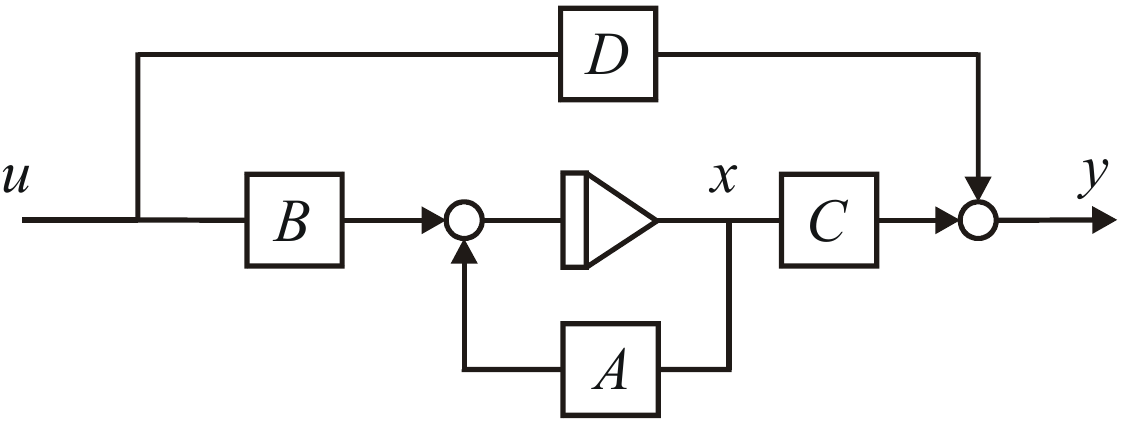
\includegraphics[width = 0.85\linewidth]{img/state-space-models/LTI-state-space-model.png}
    \caption{Representação em Diagrama de Blocos do Modelo em Espaço de Estados (LIT).}
    \label{fig:LTI-state-space-model}
\end{figure}

%//==============================--A--==============================//%
\newpage
\subsubsection[1.1.1 Conversão entre Modelo de Estado e Função de Transferência]{$\pmb{\rightarrow}$ Conversão entre Modelo de Estado e Função de Transferência}
\label{subsec:convertion-to-transfer}

\noindent Partindo do Modelo em Espaço de Estados da \hyperref[subsec:state-space-model]{secção anterior}\footnotemark[1]:
\begin{align*}
    \dot{\pmb{x}}(t) &= \pmb{A}\, \pmb{x}(t) + \pmb{B}\, u(t)\qquad \pmb{x}(t_0) = \pmb{x}_0 \\
    y(t) &= \pmb{C}\, \pmb{x}(t)
\end{align*}

\noindent E aplicando a Transformada de Laplace ($\mathcal{L}\{\cdot\}$) com \underline{condições iniciais nulas}, obtém-se:
$$
    \begin{cases}
        s\pmb{X}(s) = \pmb{A}\,\pmb{X}(s) + \pmb{B}\,U(s) \\
        Y(s) = \pmb{C}\, \pmb{X}(s)
    \end{cases}
$$
$$
    \therefore Y(s) = \pmb{C}\left( s\pmb{I}-\pmb{A} \right)^{-1}\pmb{B}\,U(s)
$$

\noindent E, como tal, é possível converter novamente para tempo continuo usando a Transformada de Laplace Inversa ($\mathcal{L}^{-1}\{\cdot\}$), i.e.:
$$
    y(t) = \mathcal{L}^{-1}\{\pmb{C}\left( s\pmb{I}-\pmb{A} \right)^{-1}\pmb{B}\,U(s)\}
$$

\vspace{-0.5em}
{
\mdfsetup{linewidth=2pt}

\begin{mdframed}
    \noindent Esta análise também permite definir a \underline{Função de Transferência} (relação da entrada com a saída):
    
    \vspace{-0.5em}
    $$
        G(s) \delequal \frac{Y(s)}{U(s)} = \pmb{C}\left( s\pmb{I}-\pmb{A} \right)^{-1}\pmb{B},
    $$
\end{mdframed}
}

\noindent em que
$$
    \left( s\pmb{I}-\pmb{A} \right)^{-1} = \frac{\text{adj}\left[(s\pmb{I}-\pmb{A}) \right]}{\det\left[( s\pmb{I}-\pmb{A}) \right]}
$$

{
\mdfsetup{linewidth=2pt}

\begin{mdframed}
    \noindent $\pmb{\rightarrow}$ \textbf{\textit{Nota}:} As soluções obtidas resultam do facto da \underline{condição inicial ser nula}. Caso não se verificasse, não seria possível deduzir uma Função de Transferência, e ter-se-ia ainda:
    \vspace{-0.5em}
    $$
        y(t) = \mathcal{L}^{-1}\{\pmb{C}\left( s\pmb{I}-\pmb{A} \right)^{-1}\cdot(\pmb{x}_0+\pmb{B}\,U(s))\}
    $$
    \vskip -0.5em
    \hfill\ensuremath{\Box}
\end{mdframed}
}

\footnotetext[1]{Daqui em diante, assume-se $\pmb{D} \equiv \pmb{0}$.}
%//==============================--B--==============================//%
\vspace{-1em}
\subsubsection[1.1.2 Pólos e Zeros]{$\pmb{\rightarrow}$ Pólos e Zeros}
\label{subsec:poles-and-zeroes}

\noindent Ao analisar a Função de Transferência, é possível observar os pólos e os zeros.
\begin{enumerate}
    \item[$\blacktriangle$] Os pólos são, por definição, as raízes do \underline{denominador de $G(s)$}, o chamado polinómio característico:
\end{enumerate}
\vspace{-0.5em}
$$
    \det\left[( s\pmb{I}-\pmb{A}) \right] = 0
$$

\noindent Os pólos, neste caso, \underline{apenas} dependem da Matriz da Dinâmica. 

\begin{enumerate}
    \item[$\blacktriangle$] Os zeros são, por definição, as raízes do \underline{numerador de $G(s)$}:
\end{enumerate}
\vspace{-0.5em}
$$
    \pmb{C}\,\text{adj}\left[(s\pmb{I}-\pmb{A}) \right]\pmb{B} = 0
$$

\noindent Note-se que os zeros dependem não só da Matriz da Dinâmica mas também das Matrizes de Entrada e de Saída.
%//==============================--C--==============================//%
\newpage
\subsubsection[1.1.3 Obtenção do Modelo de Estado através da Função de Transferência]{$\pmb{\rightarrow}$ Obtenção do Modelo de Estado através da Função de Transferência}
\label{subsec:transfer-to-model}

\noindent Tendo a Função de Transferência é possível obter o Modelo de Estado. Este modelo não é único, existem infinitas realizações de modelos, que podem ser obtidas umas das outras através de transformações.

%%%%%
\paragraph[1.1.3 a) Sistema sem Zeros]{$\pmb{\star}$ Sistema sem Zeros:}\mbox{}\\
\noindent Neste caso a Função de Transferência é do tipo:
$$
    G(s) = \frac{b_0}{s^n + a_1 s^{n-1} + \dots + a_{n-1} s + a_n}
$$

\noindent Uma realização possível é utilizar as variáveis de fase, i.e., começar por definir os estados (fases) como sendo:
\vspace{-0.5em}
\begin{align*}
    x_1(t) &= y(t) \\
    x_2(t) &= \dot{x}_1(t) = \dot{y}(t) \\
           &\mkern9mu\vdots \\
    x_n(t) &= \dot{x}_{n-1}(t) = y^{(n-1)}(t)
\end{align*}

\noindent E como tal, a derivada a última variável de fase é dada por:
$$
    \dot{x}_n(t) = y^{(n)}(t) = -a_1 x_n(t) - a_2 x_{n-1}(t) \hdots - a_{n-1} x_1(t) + b_0 u(t)
$$

\noindent Ou seja, temos a Matriz da Dinâmica na \underline{forma companheira} e podemos definir um Modelo de Estados da seguinte forma:
$$
    \dot{\pmb{x}}(t) = 
    \begin{bmatrix} 
        0 & 1 & \dots & 0 & 0\\
        0 & 0 & 1 & \dots & 0\\
        \vdots &  &  & \ddots & \vdots\\
        0 & 0 & \dots & 0 & 1\\
        -a_n & -a_n & \dots & -a_2 & -a_1 
    \end{bmatrix} \pmb{x}(t) 
    + 
    \begin{bmatrix} 
        0\\
        0\\
        \vdots\\
        0\\
        b_0
    \end{bmatrix}
    u(t)
$$

\noindent E a Equação de Saída como:
$$
    y(t) = 
    \begin{bmatrix}
        1 & 0 & \dots & 0    
    \end{bmatrix}
    \pmb{x}(t)
$$

%%%%%
\paragraph[1.1.3 b) Sistema com Zeros]{$\pmb{\star}$ Sistema com Zeros:}\mbox{}\\
Neste caso a Função de Transferência é do tipo:
$$
    G(s) = \frac{b_1 s^{n-1} + b_2 s^{n-2} + \dots + b_n}{s^n + a_1 s^{n-1} + \dots + a_{n-1} s + a_n}
$$

\noindent (a equação anterior é assim definida para sistemas causais.)

É possível definir o sistema como uma parte sem zeros e outra com zeros:
\begin{enumerate}
    \item[$\blacktriangle$] Parte sem zeros: $X_1(s) = \dfrac{1}{s^n + a_1 s^{n-1} + \dots + a_{n-1} s + a_n}\cdot U(s)$
    \item[$\blacktriangle$] Parte com zeros: $Y(s) = X_1(s) \cdot (b_1 s^{n-1} + b_2 s^{n-2} + \dots + b_n)$
\end{enumerate}

\begin{figure}[H]
    \centering
    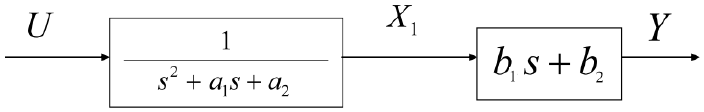
\includegraphics[width = 0.85\linewidth]{img/state-space-models/transfer-decomposition.png}
    \caption{Decomposição do sistema (LIT) numa parte com e noutra sem zeros.}
    \label{fig:transfer-decomposition}
\end{figure}

\noindent A parte \underline{sem zeros} resulta em:
$$
    \dot{\pmb{x}}(t) = 
    \begin{bmatrix} 
        0 & 1 & \dots & 0 & 0\\
        0 & 0 & 1 & \dots & 0\\
        \vdots &  &  & \ddots & \vdots\\
        0 & 0 & \dots & 0 & 1\\
        -a_n & -a_n & \dots & -a_2 & -a_1 
    \end{bmatrix} \pmb{x}(t) 
    + 
    \begin{bmatrix} 
        0\\
        0\\
        \vdots\\
        0\\
        1
    \end{bmatrix}
    u(t)
$$

\noindent E, finalmente, a parte \underline{com zeros} leva a que:
$$
    y(t) = 
    \begin{bmatrix}
        b_n & b_{n-1} & \dots & b_2 & b_1    
    \end{bmatrix}
    \pmb{x}(t)
$$

{
\mdfsetup{linewidth=2pt}

\begin{mdframed}
    \noindent $\pmb{\rightarrow}$ \textbf{\textit{Nota}:} No sistema com zeros a Matriz da Dinâmica manteve-se constante!
\end{mdframed}
}

%//==============================--D--==============================//%
\subsubsection[1.1.4 A equação homogénea e Notas sobre Álgebra Linear]{$\pmb{\rightarrow}$ A equação homogénea}
\label{subsec:homogeneous-equation}

Relaxando o Modelo do sistema para que contenha apenas a Matriz da Dinâmica, obtém-se um Sistema mais simples. A solução desta equação desempenha um papel fundamental na solução da equação de estado (de \hyperref[subsec:non-homogeneous-equation]{sistemas lineares com entrada}) e na compreensão da
dinâmica local de muitos sistemas não lineares. 

A estrutura da solução depende dos \underline{valores próprios} e dos \underline{vetores próprios} de $\pmb{A}$. Assim:
\vspace{0em}
$$
    \dot{\pmb{x}}(t) = \pmb{A}\, \pmb{x}(t)\qquad \pmb{x}(t_0) = \pmb{x}_0 \\
$$

{
\mdfsetup{linewidth=2pt}

\begin{mdframed}
    \noindent $\pmb{\rightarrow}$ \textbf{\textit{Notas sobre Álgebra Linear}:}
    
    \noindent Sendo $\pmb{A}$ quadrada $[n \times n]$, é possível chegar à seguinte igualdade:
    
    \vspace{0em}
    $$
        \pmb{A}\, \pmb{v}_i = \lambda_i\, \pmb{v}_i
    $$

    \begin{enumerate}
        \item[$\blacktriangle$] \textbf{Valores próprios:} $\lambda_i$ são as soluções de $\det[(\lambda\pmb{I}-\pmb{A})] = 0$.

        \item[$\blacktriangle$] \textbf{Vetores próprios:} $\pmb{v}_i$ são as soluções de $(\lambda_i\pmb{I}-\pmb{A})\pmb{v}_i = 0$ (são definidos a menos de uma razão de normalização).
    \end{enumerate}

    \noindent Em que $\pmb{v}_i$ também se pode denominar por \underline{vetor de modo}. Geralmente existem (podem não existir) $n$ vetores próprios linearmente independentes. Caso existam podemos utilizar a \underline{diagonalização de matrizes} para resolver a equação homogénea (veremos em seguida).
\end{mdframed}
}

\newpage

{
\mdfsetup{linewidth=2pt}

\begin{mdframed}
    \noindent $\pmb{\rightarrow}$ \textbf{\textit{Diagonalização de matrizes}:}

    \noindent Tendo $n$ vetores próprios linearmente independentes então é possível definir a Matriz Modal $[n \times n]$, não singular (admite inversa):
    $$
        \pmb{M} = 
        \begin{bmatrix}
                \pmb{v}_1 & \pmb{v}_2 & \dots & \pmb{v}_n
        \end{bmatrix}
    $$

    \noindent Tendo também $n$ valores próprios podemos definir uma Matriz Diagonal $[n \times n]$, que tem os valores próprios na sua diagonal principal:
    $$
        \pmb{\Lambda} \delequal \text{diag}(\lambda_1,\dots,\lambda_n) = 
        \begin{bmatrix}
                \lambda_1 & 0 & \dots & 0 \\
                0 & \lambda_2 & \dots & 0 \\
                0 & 0 & \ddots & 0 \\
                0 & 0 & \dots & \lambda_n 
        \end{bmatrix}
    $$

    \noindent Assim, podemos escrever:
    $$
        \pmb{A}\, \pmb{M} = \pmb{M}\,\pmb{\Lambda} \implies
        \begin{cases}
            \pmb{A} = \pmb{M}\, \pmb{\Lambda}\, \pmb{M}^{-1}\\
            \pmb{\Lambda} = \pmb{M}^{-1}\, \pmb{A}\, \pmb{M}
        \end{cases}
    $$
\end{mdframed}
}

\noindent Podemos então fazer uma transformação ao \underline{modelo da equação homogénea} em que se rodam as coordenadas para as coordenadas ortogonais definidas pelos vetores próprios:
$$
    \pmb{x}(t) = \pmb{M}\, \pmb{z}(t) \iff \pmb{z}(t) = \pmb{M}^{-1}\,\pmb{x}(t)
$$

\noindent Como:
$$
    \pmb{\dot{z}}(t) = \pmb{M}^{-1}\,\pmb{\dot{x}}(t) = \pmb{M}^{-1}\,\pmb{A}\,\pmb{x}(t) = \pmb{M}^{-1}\,\pmb{A}\,\pmb{M}\, \pmb{z}(t)
$$

\noindent Vem que:
$$
    \pmb{\dot{z}}(t) = \pmb{\Lambda}\, \pmb{z}(t)
$$

\noindent em que $\pmb{\Lambda}$ é a Matriz Diagonal---definida acima---que contém os valores próprios.
\\[6pt]
\noindent Ficamos com um sistema facilmente resolúvel:
$$
    \begin{cases}
        \dot{z}_1(t) = \lambda_1 z_1(t)\\
        \mkern46mu \vdots\\
        \dot{z}_n(t) = \lambda_n z_n(t)
    \end{cases}
$$

\noindent Cuja solução (\textbf{que depende das condições iniciais}) é dada por:
$$
    \begin{cases}
        z_1(t) = k_1 e^{\lambda_1 t}\\
        \mkern46mu \vdots\\
        z_n(t) = k_n e^{\lambda_n t}
    \end{cases}
$$

\noindent Nas coordenadas originais $\pmb{x}(t)$, verificamos então (\textbf{Decomposição Modal}):
$$
    \pmb{x}(t) = \pmb{M}\, \pmb{z}(t) = 
    \begin{bmatrix}
        \pmb{v}_1 & \hdots & \pmb{v}_n
    \end{bmatrix}
    \begin{bmatrix}
        k_1 e^{\lambda_1 t}\\
        \vdots\\
        k_n e^{\lambda_n t}
    \end{bmatrix}
    = k_1 \pmb{v}_1 e^{\lambda_1 t} + \dots + k_n \pmb{v}_n e^{\lambda_n t} = \sum_{i=1}^{n} k_i \pmb{v}_i e^{\lambda_i t}
$$

\noindent Em que temos os $n$ \underline{modos do sistema}:
$$
    \pmb{v}_i e^{\lambda_i t}
$$

\hfill\ensuremath{\Box}

%//==============================--D--==============================//%
\subsubsection[1.1.5 Resposta no tempo de um SLIT não homogéneo (solução geral)]{$\pmb{\rightarrow}$ Resposta no tempo de um SLIT não homogéneo (solução geral)}
\label{subsec:non-homogeneous-equation}

Nos \underline{sistemas não homogéneos} o estado não evolui livremente, i.e., não é apenas afetado pela dinâmica do sistema, mas também por uma entrada. Neste caso, a solução obtém-se através da solução da \hyperref[subsec:homogeneous-equation]{equação homogénea} recorrendo ao \textbf{Princípio da Sobreposição}---tendo em conta a função de entrada $u(t)$.
\\[6pt]
\noindent Sendo o sistema descrito pela equação de estado:
$$
    \dot{\pmb{x}}(t) = \pmb{A}\, \pmb{x}(t) + \pmb{B}\, \pmb{u}(t)\qquad \pmb{x}(t_0) = \pmb{x}_0
$$

\noindent Obtém-se a evolução temporal:
{
\mdfsetup{linewidth=2pt}

\begin{mdframed}
    \noindent $\pmb{\rightarrow}$ \textbf{\textit{Fórmula da Variação das Constantes}:}
    $$
        \pmb{x}(t) = \underbrace{e^{\pmb{A}(t-t_0)}\, \pmb{x}_0}_{\text{Regime Livre}} + \underbrace{e^{\pmb{A}(t-t_0)} \int_{t_0}^{t} e^{\pmb{A}(t_0-s)} \pmb{B} u(s)\, ds}_{\text{Regime Forçado}}
    $$
    
\end{mdframed}
}

\noindent Relembrando a Análise Diferencial, trivialmente se obtém a exponencial da Matriz da Dinâmica (Matriz de Transição). 

{
\mdfsetup{linewidth=2pt}

\begin{mdframed}
    \noindent $\pmb{\rightarrow}$ \textbf{\textit{Notas sobre Análise Diferencial}:}
    \begin{itemize}
        \item[$\blacktriangle$] \textbf{Exponencial de uma matriz:}
            \vspace{-0.5em}
            $$
                e^{\pmb{A}(t-t_0)} \delequal \pmb{I} + \pmb{A}(t-t_0) + \frac{1}{2!}\pmb{A}^2(t-t_0)^2 + \dots = \sum_{n=0}^{+\infty} \frac{\pmb{A}^n(t-t_0)^n}{n!}
            $$

        \vspace{-1em}
        \item[$\blacktriangle$] \textbf{Cálculo de} $e^{\pmb{A}t}$ \textbf{caso a matriz seja diagonalizável:}
            \vspace{-0.5em}
            $$
                e^{\pmb{A}t} = \pmb{M}\, e^{\pmb{\Lambda}t}\, \pmb{M}^{-1}
            $$
            
            \vspace{-1.0em}
            \noindent em que $e^{\pmb{\Lambda}t} \delequal \text{diag}(e^{\lambda_1 t}, \dots, e^{\lambda_n t})$.

            \item[$\blacktriangle$] \textbf{Cálculo de} $e^{\pmb{A}t}$ \textbf{através da Transformada de Laplace:}
            
            \noindent Aplicando a Transformada de Laplace à equação homogénea:
            $$
                s\pmb{X}(s) - \pmb{x}_0 = \pmb{A}\,\pmb{X}(s) \iff \pmb{X}(s) = \left( s\pmb{I} -\pmb{A} \right)^{-1} \pmb{x}_0
            $$
            
            \vspace{-0.5em}
            \noindent Aplicando a Transformada Inversa:
            
            \vspace{-0.5em}
            $$
                \pmb{x}(t) = \mathcal{L}^{-1}\{\left( s\pmb{I} -\pmb{A} \right)^{-1}\}\vert_{t-t_0}\, \pmb{x}_0
            $$

            \vspace{-0.5em}
            \noindent Desta forma:
            $$
                e^{\pmb{A}(t-t_0)} \delequal \mathcal{L}^{-1}\{\left( s\pmb{I} -\pmb{A} \right)^{-1}\}\vert_{t-t_0}
            $$

            \vspace{-1em}
            \item[$\blacktriangle$] \textbf{(...)}
    \end{itemize}
    
\end{mdframed}
}

%//==============================--@--==============================//%
\newpage
\subsection[1.2 Análise da Função de Transferência do Modelo de Estados]{$\rightarrow$ Análise da Função de Transferência do Modelo de Estados}
\label{subsec:model-analysis}

\phantomsection\addcontentsline{toc}{subsubsection}{1.2.1 Teoremas do valor inicial e final}

Se $f(t)$ não contiver impulsos ou singularidades de ordem superior na origem e convergir para um valor constante quando $t \to +\infty$, então, aplicam-se os teoremas:
\begin{center}%
    \begin{tabular}{c c}%
        \begin{minipage}{0.425\linewidth}%
            \begin{theo}[\underline{Teorema do Valor Incial}]{teo:inicial-value}\label{teo:inicial-value}
                $$
                    \lim_{t \to 0} f(t) = \lim_{s \to +\infty} sF(s)
                $$
            \end{theo}%
        \end{minipage}%
        &%
        \begin{minipage}{0.425\linewidth}%
            \begin{theo}[\underline{Teorema do Valor Final}]{teo:final-value}\label{teo:final-value}
                $$
                    \lim_{t \to +\infty} f(t) = \lim_{s \to 0} sF(s)
                $$
            \end{theo}%
        \end{minipage}%
    \end{tabular}%
\end{center}%

\subsubsection[1.2.2 Resposta ao escalão unitário de sistemas LIT]{$\pmb{\rightarrow}$ Resposta ao escalão unitário de sistemas LIT}

\begin{figure}[H]
    \centering
    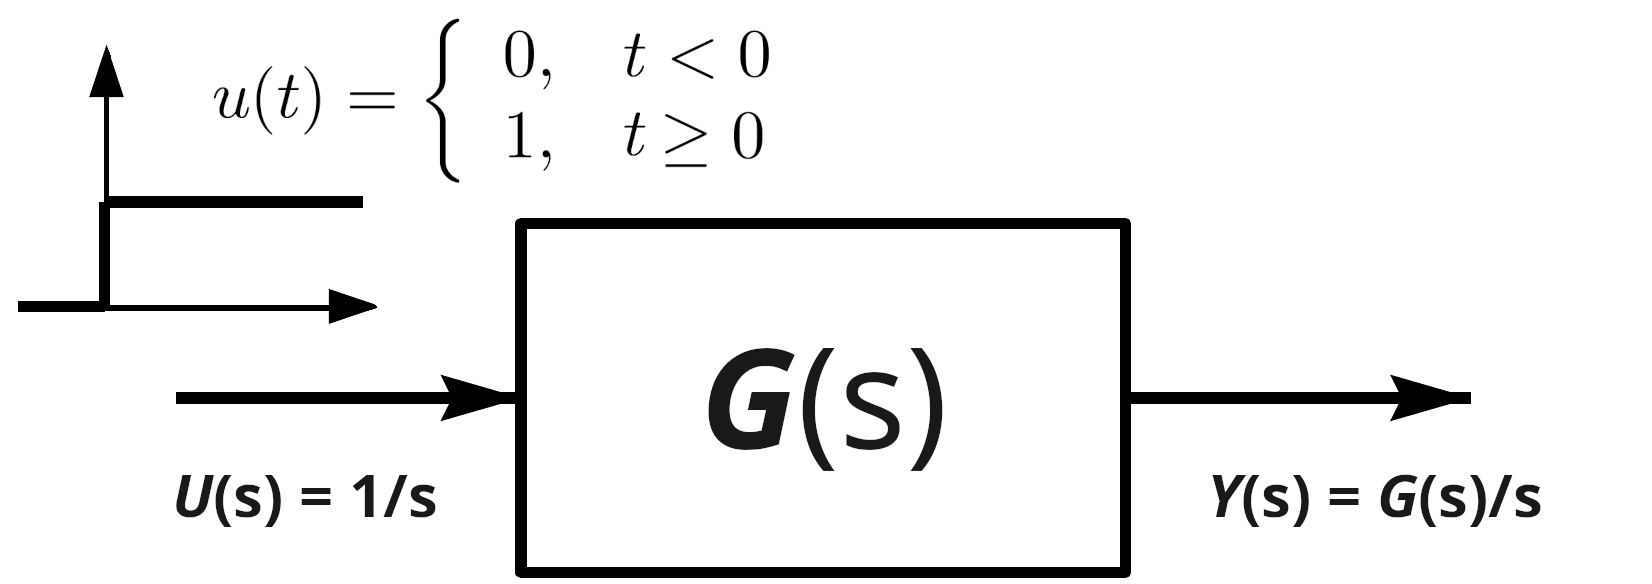
\includegraphics[width = 0.5\linewidth]{img/state-space-models/unit-step-response.png}
    \caption{Resposta do sistema ao degrau unitário.}
    \label{fig:unit-step-response}
\end{figure}

{
\mdfsetup{linewidth=2pt}

\begin{mdframed}
    \begin{itemize}
    \item[$\blacktriangle$] \underline{Valor final da resposta} ao escalão unitário:
        
        \vspace{-1em}
        $$
            \lim_{t \to +\infty} y(t) = \lim_{s \to 0} sY(s) = \lim_{s \to 0} s\frac{G(s)}{s} = G(0)
        $$
        
    \vspace{-0.5em}
    \item[$\blacktriangle$] \underline{Valor inicial da resposta} ao escalão:
        
        \vspace{-1em}
        $$
            \lim_{t \to 0} y(t) = \lim_{s \to +\infty} sY(s) = \lim_{s \to +\infty} s\frac{G(s)}{s} = \lim_{s \to +\infty} G(s)
        $$
        
    \vspace{-0.5em}
    \item[$\blacktriangle$] \underline{Valor inicial da derivada da resposta} ao escalão unitário:
        
        \vspace{-1em}
        $$
            \lim_{t \to 0} \dot{y}(t) = \lim_{s \to +\infty} s\, (sY(s)) = \lim_{s \to +\infty} s^2\frac{G(s)}{s} = \lim_{s \to +\infty} sG(s)
        $$

    \vspace{-0.5em}
    \item[$\blacktriangle$] \underline{Valor final da derivada da resposta} ao escalão unitário:
        
        \vspace{-1em}
        $$
            \lim_{t \to +\infty} \dot{y}(t) = \lim_{s \to 0} s\, (sY(s)) = \lim_{s \to 0} s^2\frac{G(s)}{s} = \lim_{s \to 0} s G(s)
        $$
    \end{itemize}
\end{mdframed}
}

\vspace{-1em}
\paragraph[1.2.2.1 Excesso de pólos-zeros]{$\pmb{\star}$ Excesso de polos-zeros (resposta ao escalão unitário)}\mbox{}\\
\begin{center}%
    \begin{tabular}{c c}%
        \begin{minipage}{0.425\linewidth}%
            \vspace{-1em}
            \begin{mdframed}
                $$
                    \lim_{t \to 0} y(t) = \lim_{s \to +\infty} G(s)
                $$
            \end{mdframed}
        \end{minipage}%
        &%
        \begin{minipage}{0.425\linewidth}%
            \vspace{-1em}
            \begin{mdframed}
                $$
                    \lim_{t \to 0} \dot{y}(t) = \lim_{s \to +\infty} sG(s)
                $$
            \end{mdframed}
        \end{minipage}%
    \end{tabular}%
\end{center}%

{\setlength{\tabcolsep}{16pt}
\begin{center}
    \begin{tabular}{p{0.4\textwidth} | p{0.4\textwidth}}
        \centerline{\underline{$\#\textbf{pólos} > \#\textbf{zeros}$}} & \centerline{\underline{$\#\textbf{pólos} > \#\textbf{zeros}+1$}} \\[-14pt]
        Resposta ao escalão contínua & Derivada da resposta contínua \\[4pt]
        \centerline{\underline{$\#\textbf{pólos} = \#\textbf{zeros}$}} & \centerline{\underline{$\#\textbf{pólos} = \#\textbf{zeros}+1$}} \\[-14pt]
        Resposta descontínua, com salto finito & Derivada da resposta descontínua, mas finita \\[4pt]
        \centerline{\underline{$\#\textbf{pólos} < \#\textbf{zeros}$}} & \centerline{\underline{$\#\textbf{pólos} < \#\textbf{zeros}+1$}} \\[-14pt]
        Resposta descontínua, com salto infinito & Derivada da resposta descont.,  infinita \\
        \bottomrule
    \end{tabular}
\end{center}
}

\renewcommand*{\thefootnote}{\fnsymbol{footnote}}
\footnotetext[4]{\underline{\textbf{Nota:}} caso um dos zeros se encontre no SPD, então temos um sistema de \underline{fase não mínima}.}
\renewcommand*{\thefootnote}{\arabic{footnote}}

%//==============================--C--==============================//%
\subsubsection[1.2.3 Sistemas de 2\textordfeminine{} ordem (sem zeros)]{$\pmb{\rightarrow}$ Sistemas de 2\textordfeminine{} ordem (sem zeros)}

$$
    G(j\omega) = \frac{\omega_n^2}{s^2 + 2\zeta\omega_ns + \omega_n^2}
$$

\begin{mdframed}
    \noindent $\zeta$ - Determina a forma da resposta.\\
    \noindent $\omega_n$ - Determina a escala de tempo.\\ 
    \noindent Quando maior for $\omega_n$ maior é a largura de banda e mais rápido é o sistema.
\end{mdframed}

\vspace{-0.5em}
\begin{figure}[H]
    \label{fig:second-order-system-step-response}
    \begin{subfigure}[b]{0.5\linewidth}
        \centering
        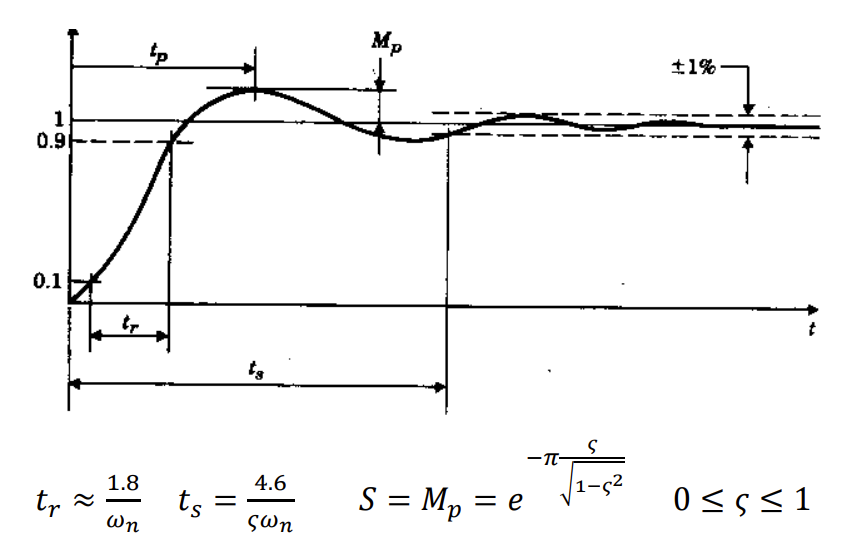
\includegraphics[width=0.8\linewidth]{img/state-space-models/second-order-system-step-response.png}
        \label{fig:second-order-step-response} 
    \end{subfigure}
    \begin{subfigure}[b]{0.5\linewidth}
        \centering
        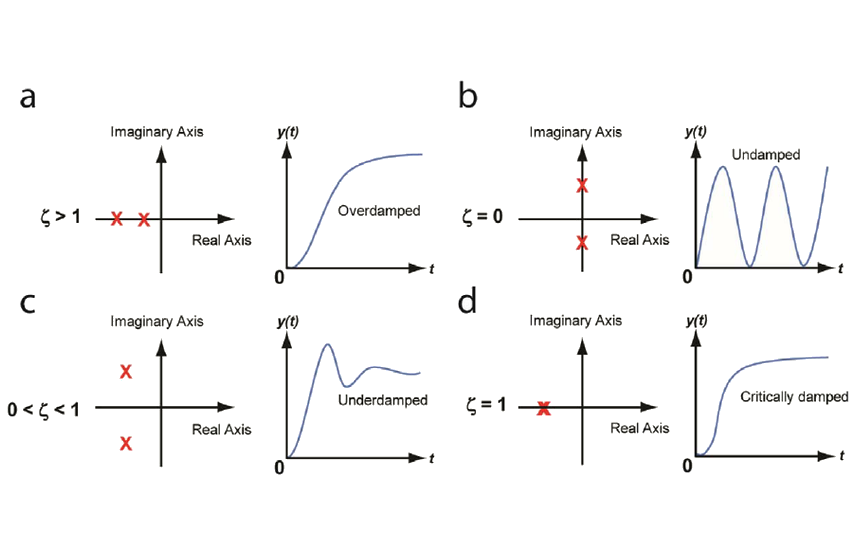
\includegraphics[width=0.85\linewidth]{img/state-space-models/step-response-second-order-system.png} 
        \label{fig:second-order-dif-cases} 
    \end{subfigure}
    \begin{minipage}{1\linewidth}
        \vspace{-1.5em}
        \caption{Tipos de resposta de sistemas de segunda ordem sem zeros ($\star$ resposta ao escalão unitário).}
    \end{minipage}
\end{figure}

%//==============================--D--==============================//%
\subsubsection[1.2.4 Diagramas de Bode]{$\pmb{\rightarrow}$ Diagramas de Bode}

``The most useful technique for hand plotting was developed by H. W. Bode at Bell Laboratories between 1932 and 1942. The idea in Bode's method is to plot magnitude curves using a logarithmic scale and phase curves using a linear scale. This strategy allows us to plot a high-order $G(j\omega)$ by simply adding the separate terms graphically.
$$
    \frac{\bar{s}_1 \bar{s}_2}{\bar{s}_3 \bar{s}_4 \bar{s}_5} = \frac{r_1 e^{j\theta_1} r_2 e^{j\theta_2}}{r_3 e^{j\theta_3} r_4 e^{j\theta_4} r_5 e^{j\theta_5}} =
    \left( \frac{r_1 r_2}{r_3 r_4 r_5} \right) e^{j(\theta_1 + \theta_2 - \theta_3 - \theta_4 - \theta_5)}
$$
phases of the individual terms are added directly to obtain the phase of the composite expression, $G(j\omega)$. Furthermore, because
$$
    \vert G(j\omega) \vert = \frac{r_1 r_2}{r_3 r_4 r_5}
$$
it follows that
$$
    \log_{10}\vert G(j\omega) \vert = \log_{10}(r_1) + \log_{10}(r_2) - \log_{10}(r_3) - \log_{10}(r_4) - \log_{10}(r_5).\text{''\cite{FranklinPowell2015}}
$$

\begin{figure}[H]
    \centering
    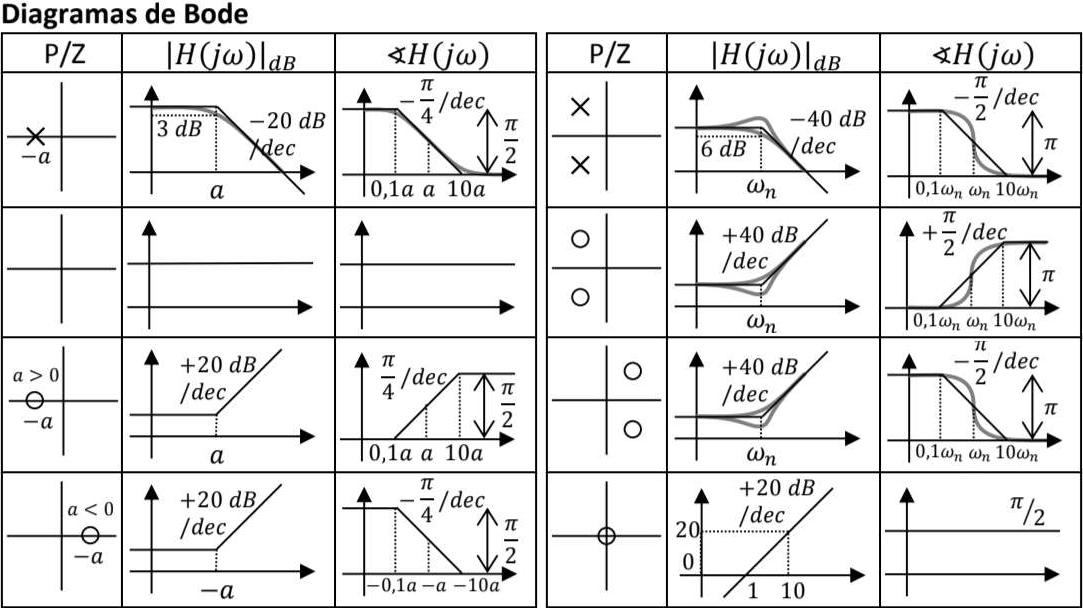
\includegraphics[width = 0.7\linewidth]{img/state-space-models/bode.png}
    \caption{Resposta assimtótica---resposta em diagramas de Bode.}
    \label{fig:bode}
\end{figure}

%Adoro-te cutie 
%cutie :3 adoro-te
%//==============================--@--==============================//%